The back-end readout card for the system under development, the Zynq UltraScale+ RFSoC ZCU216 Evaluation Card, was chosen taking into consideration the points described in \autoref{sec:selection}.
In this section, the overall architecture and features of the card are presented.
A possibility for evaluation of the card is also demonstrated.
At last, a design for the read-out firmware is proposed. 

\section{Xilinx Zynq UltraScale+ RFSoC ZCU216 Evaluation Card}
Zynq UltraScale+ RFSoCs: Combine RF data converter subsystem and forward error correction with industry-leading
programmable logic and heterogeneous processing capability. Integrated RF-ADCs, RF-DACs, and soft decision FECs (SD-FEC)
provide the key subsystems for multiband, multi-mode cellular radios and cable infrastructure


With the data converters integrated directly into the \gls{fpga} using parallel interfaces, they do not require the
prohibitively high-pin-count external connections needed for discrete parallel interface converters, allowing more converter

\begin{itemize}[noitemsep]
	\item Sixteen 14-bit, 2.5GSPS RF-ADC
	\item Sixteen 14-bit, 10GSPS RF-DAC
	\item I/O expansion options – FPGA Mezzanine Card (FMC+) interfaces, RFMC 2.0 interfaces, and Pmod connections
\end{itemize}
\begin{figure}[tbh]
	\centering
	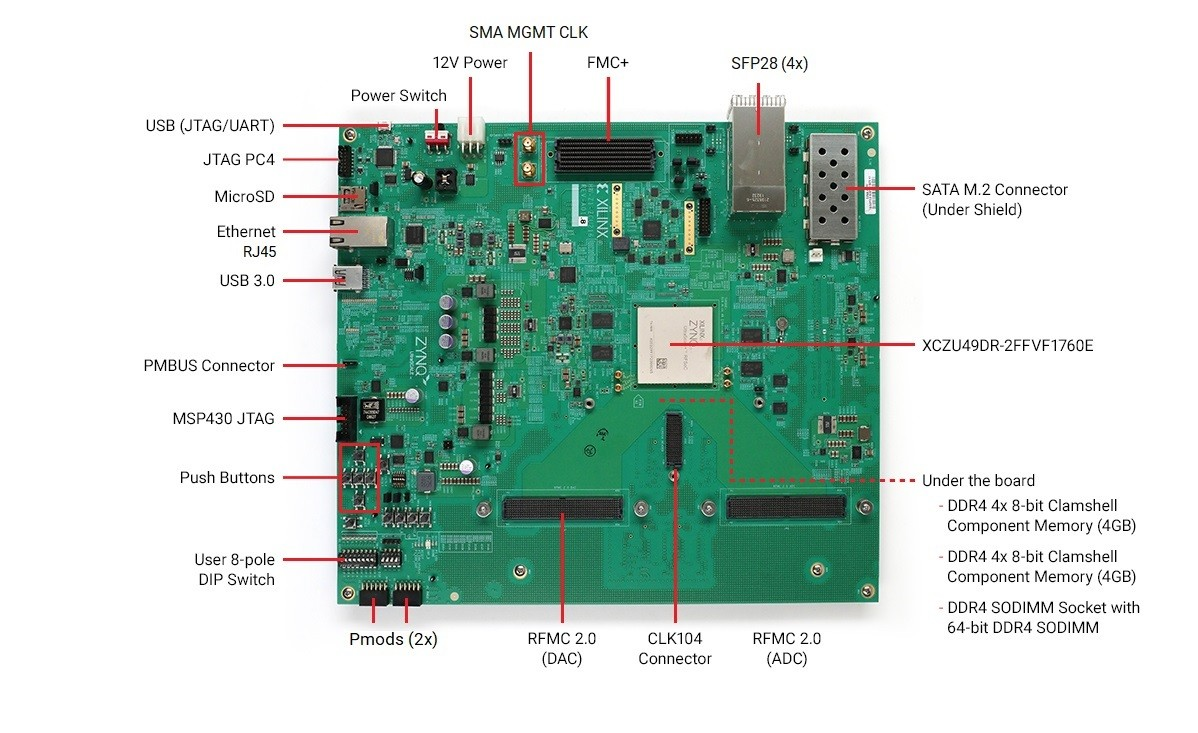
\includegraphics[width = \textwidth]{chap/04-work/img/zcu216}
	\caption{ZCU216 evaluation board}
	\label{fig:zcu216}
\end{figure}

\begin{figure}[tbh]
	\centering
	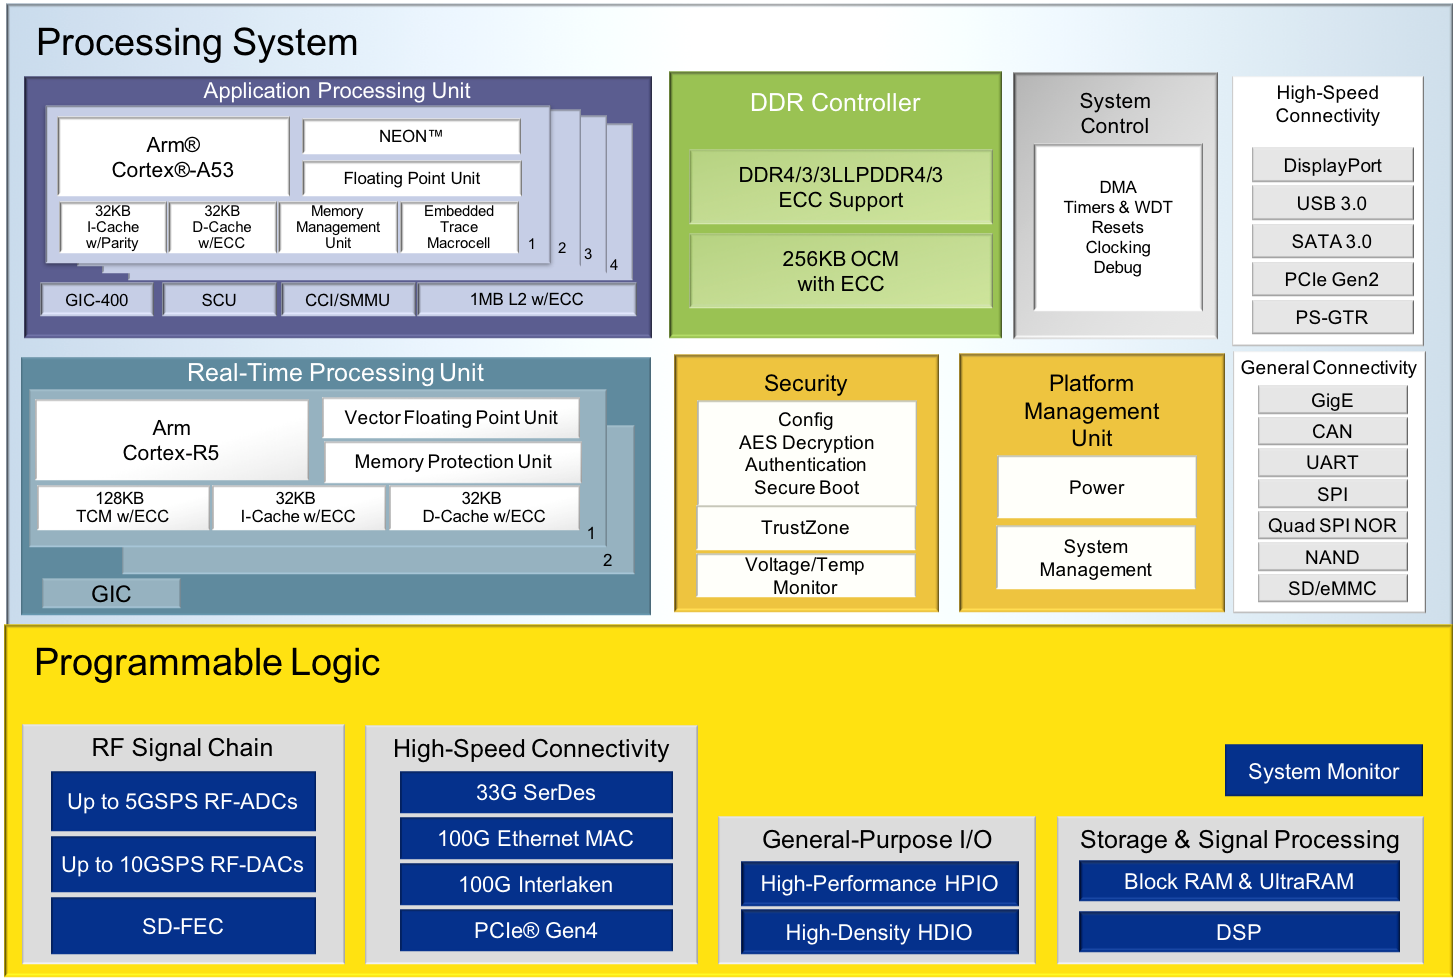
\includegraphics[width = \textwidth]{chap/04-work/img/rfsoc_blockdiagram}
	\caption{RFSoC block diagram}
	\label{fig:rfsoc}
\end{figure}
\paragraph{Evaluation Tool}
\section{Firmware}
\subsection{RF Data Converter}
\subsection{SoC}
\subsection{RDMA over Converged Ethernet (RoCE)}
As its name shows, RoCE is a network protocol defined in the InfiniBand Trade Association (IBTA) standard, allowing RDMA over converged Ethernet network. Shortly, it can be regarded as the application of RDMA technology in hyper-converged data centers, cloud, storage, and virtualized environments. It possesses all the benefits of RDMA technology and the familiarity of Ethernet.

Types of RoCE
Generally, there are two RoCE versions: RoCE v1 and RoCE v2. It depends on the network adapter or card used.

RoCE v1: The RoCE v1 protocol is an Ethernet link layer protocol allowing two hosts in the same Ethernet broadcast domain (VLAN) to communicate. It uses Ethertype 0x8915, which limits the frame length as 1500 bytes for a standard Ethernet frame and 9000 bytes for an Ethernet jumbo frame.

RoCE v2: The RoCE v2 protocol overcomes the limitation of version 1 being bounded to a single broadcast domain (VLAN). By changing the packet encapsulation to include IP and UDP headers, RoCE v2 can now be used across both L2 and L3 networks. This enables Layer 3 routing, which brings RDMA to network with multiple subnets for great scalability. Therefore, RoCE v2 is also regarded as Routable RoCE (RRoCE). Owing to the arrival of RoCE v2, the IP multicast is now also possible.
\subsection{System Integration}


